% !TEX root = ../template.tex
\chapter{Reactor Continuo Flujo Pistón}
\begin{flushleft}
    Se analiza ahora el reactor continuo de flujo de pistón (PFR). Al igual que en otros reactores, su estudio se realiza en tres casos: isotermo, adiabático y no isotermo no adiabático, obteniendo en cada uno las ecuaciones de diseño correspondientes.
    \vspace{1em}
    El PFR presenta una configuración tubular, donde existen perfiles de concentración y temperatura a lo largo del reactor. A diferencia de los reactores de mezcla perfecta, no hay homogeneización global.
    \vspace{1em}
    Por ello, los balances de materia y energía no se pueden plantear sobre todo el volumen, sino sobre un elemento diferencial de volumen $dV$, donde las condiciones pueden considerarse uniformes.
    \vspace{1em}
    Así, el modelo del reactor se obtiene a partir de balances diferenciales aplicados a un elemento de volumen del reactor.
\end{flushleft}
\begin{figure}[H]
    \centering
    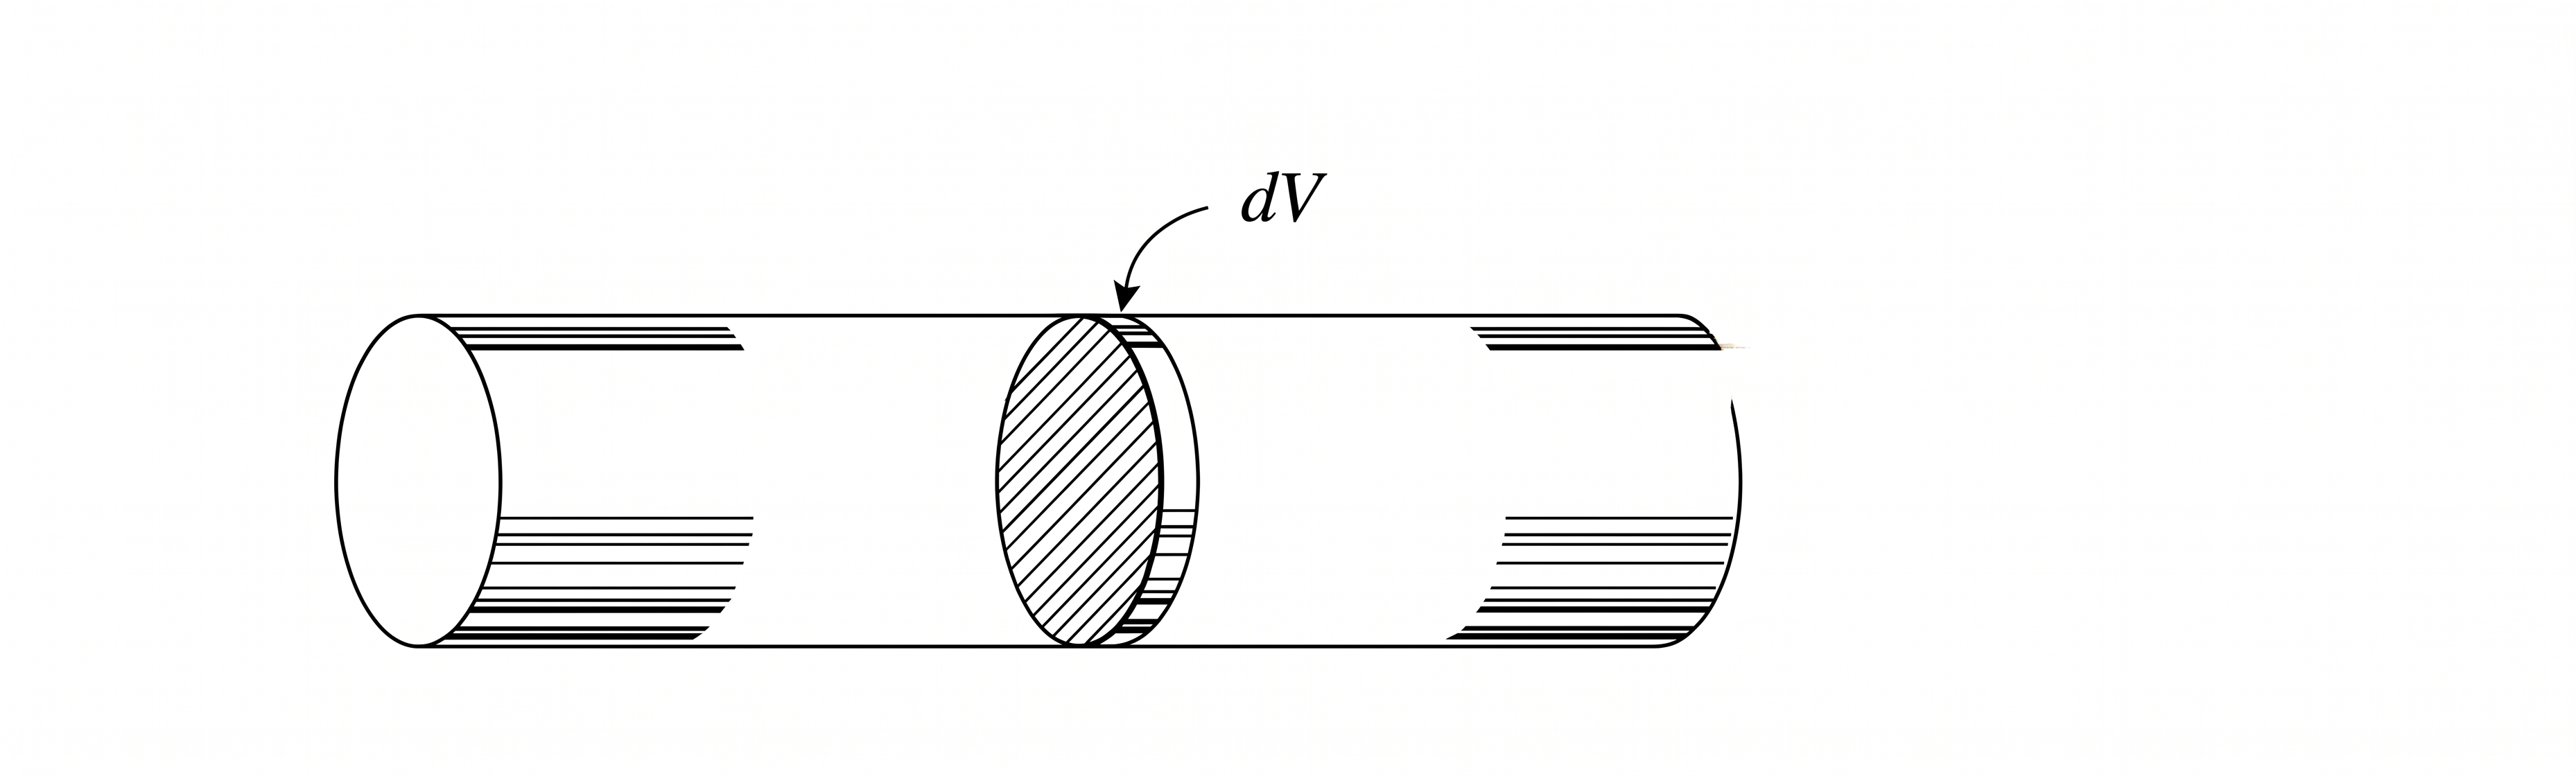
\includegraphics[width=0.75\textwidth]{Imagenes/PFR.png}
    \caption{Reactor Continuo Flujo Pistón}
    \label{fig:PFR}
\end{figure}
\begin{flushleft}
    En un reactor de flujo de pistón, el elemento diferencial de volumen puede expresarse como: \[dV = A\,dz\]
    donde $dz$ es el diferencial axial y $A$ el área transversal del tubo.
    \vspace{1em}
\end{flushleft}


\section{Isotermo}
\begin{flushleft}
    En condiciones isotermas (temperatura constante), el modelo del reactor se basa únicamente en balances de materia, ya que el balance de energía no es necesario para la modelización (solo para el diseño térmico).\\
    \vspace{1em}
    Considerando una única reacción independiente $A \rightarrow P$, el análisis se centra en el reactivo limitante y en la variable conversión $X_A$.\\
    \vspace{1em}
    Por tanto, el modelo del reactor isotermo se obtiene a partir del balance de materia diferencial aplicado al reactivo $A$.
\end{flushleft}
\dfn{Balance de materia}{
    \begin{equation}
        \frac{dN_A}{dt} = \cancelto{0}{n_A} - (\cancelto{0}{n_A} + dn_A) - r_A\cdot dV \quad \text{\scriptsize en estado estacionario $\frac{dN_A}{dt}=0$} \rightarrow -dn_A = r_A\cdot dV
        \label{eq:RCFP_balance_isotermo}
    \end{equation}
}
por tanto si lo ponemos en función de la conversión queda:

\begin{equation}
    n_A = n_{AR}(1-X_A)  \rightarrow dn_A = -n_{AR}dX_A
\end{equation}
\nt{basicamente se ha derivado la definicion de conversión}
\begin{equation}
    \int_{0}^{V}dV= n_{AR}\int_{X_{A0}}^{X_{AS}}\frac{dX_A}{-r_A} \rightarrow \boxed{V = n_{AR}\int_{X_{A0}}^{X_{AS}}\frac{dX_A}{-r_A}}
    \label{eq:RCFP_V}
\end{equation}
si a esta expresión la dividimos por el caudal:
\begin{equation}
    \textcolor{darkgreen}{\frac{V}{F}} = \textcolor{blue}{\frac{n_{AR}}{F}} \int_{X_{A0}}^{X_{AS}} \frac{dX_A}{-r_A} \rightarrow \boxed{\textcolor{darkgreen}{\tau} = \textcolor{blue}{C_{AR}}\int_{X_{A0}}^{X_{AS}}\frac{dX_A}{-r_A}}
    \label{eq:RCFP_tau}
\end{equation}
\begin{flushleft}
    Aunque el reactor discontinuo de mezcla perfecta y el reactor continuo de flujo de pistón son cinéticamente equivalentes (requieren el mismo volumen para una conversión dada), presentan diferencias en productividad.

    En el reactor continuo (PFR), el tiempo característico es el tiempo espacial $\tau$, que determina directamente la producción.

    En cambio, en el reactor discontinuo, el tiempo total de proceso incluye:
    \begin{itemize}
        \item Tiempo de reacción
        \item Tiempo de carga
        \item Tiempo de descarga
        \item Tiempo de limpieza
    \end{itemize}

    Por tanto, el tiempo efectivo de producción es mayor, reduciendo la productividad.

    En consecuencia, aunque ambos reactores sean equivalentes desde el punto de vista cinético, el reactor continuo de flujo de pistón resulta más productivo al no requerir tiempos de maniobra.
\end{flushleft}

\noindent si tuviesemos r reacciones independientes y un numero de componentes i, se generalizaria a:

\begin{align}
    -dn_i           & = r_i \cdot dV                                                               \\
    F \cdot dc_i    & = -r_i \cdot dV \;=\; -r_i \cdot S \cdot dz                                  \\
    \frac{dC_i}{dz} & = -r_i \cdot \frac{S}{F}
    \;\;\leftrightarrow\;\;
    \frac{F}{S} = V    \text{\scriptsize(velocidad media de circulción de la mezcla reaccionante)} \\
    \frac{dC_i}{dz} & = -\frac{r_i}{V}
\end{align}

\section{adiabático}

\begin{flushleft}
    En el funcionamiento adiabático de un reactor de flujo de pistón (PFR), se plantean el balance de materia y el balance entálpico.

    Considerando una única reacción $A \rightarrow P$ y trabajando con la conversión $X_A$ como variable de diseño:

    \begin{itemize}
        \item El balance de materia se aplica al reactivo limitante.
        \item El balance entálpico incluye los términos de entrada, salida y generación (debido a la reacción).
    \end{itemize}
    \begin{align}
        \frac{dN_A}{dt}                   & = n_A - (n_A + dn_A) - r_A \cdot dV                                & \text{\scriptsize balance de materia} \label{eq:materia}  \\[10pt]
        \frac{d}{dt}(M \cdot c_p \cdot T) & = m \cdot c_p \cdot (T - (T + dT)) + \Delta H_A \cdot r_A \cdot dV & \text{\scriptsize balance de entalpía} \label{eq:energia}
    \end{align}
    En estado estacionario, los términos de acumulación se anulan, simplificando ambos balances.
    \begin{align}
        \frac{dN_A}{dt}                 & = - r_A \cdot dV                  &  & \text{balance de materia}  \\
        m \cdot c_p \cdot \frac{dT}{dt} & = - \Delta H_A \cdot r_A \cdot dV &  & \text{balance de entalpía}
    \end{align}
    \cor{diferencial de volumen}{
        \begin{equation}
            dV = S\cdot dz = \frac{\pi}{4}\cdot D^2\cdot dz
        \end{equation}
    }
    y el diferencial de caudal molar puede escribirse en función de la conversión.

    Al combinar ambos balances y realizar las sustituciones correspondientes, se obtiene que en condiciones adiabáticas:
    \begin{align}
        n_{AR} \cdot \textcolor{red}{dX_A} & = r_A \cdot \frac{\pi}{4}\cdot D^2\cdot \textcolor{blue}{dz}                       & \longrightarrow  \frac{\textcolor{red}{dX_A}}{\textcolor{blue}{dz}}  = \frac{r_A}{n_{AR}}     \cdot    \frac{\pi}{4}   \cdot D^2 \label{eq:RCFP_4_14} \\
        m \cdot c_p \cdot dT               & = -\Delta H_A \cdot dn_A = \Delta H_A \cdot n_{AR} \cdot dX_A \label{eq:RCFP_4_15}
    \end{align}
    Si reordenamos la Ec.~\eqref{eq:RCFP_4_15}:
    \begin{equation*}
        dT = \frac{\Delta H_{A}\cdot n_{AR}}{m \cdot c_p} \cdot dX_A \rightarrow \underbrace{\int_{T_{0}}^{T}dT}_{T-T_0} = \frac{\Delta H_{A}\cdot n_{AR}}{m \cdot c_p} \underbrace{\int_{XA0}^{X_{A}} dX_A}_{X_A-X_{A0}}
    \end{equation*}

    de esta forma si despejamos, podemos observar que queda la temperatura como una funcion de la conversión con una relación lineal:

    \begin{equation*}
        T = T_{0} + \frac{\Delta H_{A}\cdot C_{AR}}{\rho \cdot c_p} \cdot (X_A-X_{A0})
    \end{equation*}
    si de la Ec.~\eqref{eq:RCFP_4_14} despejamos $dz$, se puede calcular la longitud del reactor necesaria para una determinada conversión:

    \begin{equation*}
        dz = \frac{n_{AR}}{\frac{\pi}{4}D^2} \cdot \frac{dX_A}{r_A} \longrightarrow  \int_{0}^{L}dz = \frac{n_{AR}}{\frac{\pi}{4}D^2} \int_{X_{A0}}^{X_{AS}}\frac{dX_A}{r_A} \implies \textcolor{blue}{L} = \frac{\textcolor{darkgreen}{n_{AR}}}{\textcolor{blue}{\frac{\pi}{4}D^2}} \int_{X_{A0}}^{X_{AS}}\frac{dX_A}{r_A}
    \end{equation*}
    normalmente, mas que interesar la longitud del reactor, interesa el volumen por tanto cabe recordar que\\
    $V=\frac{\pi}{4}D^2 L$, de esta forma obtenemos:
    \begin{equation}
        \textcolor{darkgreen}{\tau} = \frac{\textcolor{blue}{V}}{\textcolor{darkgreen}{F_R}} = \frac{\textcolor{blue}{L \cdot \frac{\pi}{4}D^2}}{F_R} = \textcolor{darkgreen}{C_{AR}} \int_{X_{A0}}^{X_{AS}}\frac{dX_A}{r_A}
    \end{equation}
    Como se puede observar el cálculo del volumen (o longitud) necesario para alcanzar una conversión dada es análogo al caso del reactor discontinuo en régimen adiabático, ya que ambos son cinéticamente equivalentes.
\end{flushleft}
\newpage
\section{no isotermo}

\begin{flushleft}
    En el diseño del reactor continuo de flujo de pistón (PFR) en régimen no isotermo, ambos balances (materia y energía) están acoplados, ya que la temperatura afecta a la velocidad de reacción. El análisis se realiza mediante balances elementales de materia y energía aplicados a un diferencial de volumen $dV$.
    \begin{align}
        \frac{dn_A}{dt}                   & = \cancelto{0}{n_A} - (n_A + dn_A) - r_A \cdot dV                                               & \text{\scriptsize balance de materia}  \\[8pt]
        \frac{d}{dt}(M \cdot c_p \cdot T) & = m \cdot c_p \cdot (T - (T + dT)) + \Delta H_A \cdot r_A \cdot dV + U \cdot dS_L \cdot (T_j-T) & \text{\scriptsize balance de entalpía}
    \end{align}
    \cor{En estado estacionario, la acumulación se anula y los balances se simplifican:}{
        \begin{align}
            \frac{dN_A}{dt}                 & = -r_A \cdot dV                                               \\
            m \cdot c_p \cdot \frac{dT}{dt} & = -\Delta H_A \cdot r_A \cdot dV + U \cdot dS_L \cdot (T_j-T)
        \end{align}
    }
    \nt{el termino $dS_L$ es el área de intercambio de calor del elemento diferencial dV}
    donde de forma analoga al apartado anterior si volvemos a considerar que el diferencial del volumen es el are adel tubo por el diferencial de z, la definicion de conversion y teniendo en cuenta que el diferencial $dS_L$  quedan las siguientes expresiones:
    \begin{align}
        dV   & =  S\cdot dz = \frac{\pi}{4}\cdot D^2\cdot dz \\
        dn_A & = - n_{AR}dX_A                                \\
        dS_L & = \pi\cdot D\cdot dz
    \end{align}
    si estas ecuaciones son sustituidas en el balance de materia y en el balance entalpico, se obtienen las siguientes ecuaciones:
    \begin{align}
        n_{AR} \cdot dX_A    & = ra \cdot \frac{\pi}{4}D^2dz                                     \\
        m \cdot c_p \cdot dT & = \Delta H_A \cdot n_{AR} \cdot dX_A + U \cdot dS_L \cdot (T_j-T)
    \end{align}
    y si hacemos un ultimo paso algebraico podemos obtener nuestras ecuaciones finales:
    \begin{align}
        \frac{dX_A}{dz}\; & =\; \frac{r_A}{n_{AR}}\,\frac{\pi D^2}{4}     \\
        \frac{dT}{dz}\;   & =\; \frac{\Delta H_A}{m c_p}\,\frac{dX_A}{dz}
        + \frac{U \pi D}{m c_p}\,(T_j - T)
    \end{align}

\end{flushleft}

\section{Recirculación en el RCFP} \label{sec:RCFP_Recirculacion}

\begin{flushleft}
    Aunque no es un caso que se suela dar en la realidad, si que permite simular un grado de mezcla axial que aunque no se da en un reactor flujo de piston(reactor real con comportamiento idealizado), si que se puede dar en un reactor tubular con un comportamiento no-ideal.\\

    Para ello es importante definir la recirculación como el caudal de recirculacion respecto al caudal de salida es decir:
    \begin{equation*}
        R = \frac{\text{caudal de recirculación}}{\text{caudal de salida}}=\frac{F_R}{F}
    \end{equation*}

    En la siguiente imagen se puede ver de una forma mas esquematica como funciona este sistema que nos ayudara a entender los balances de materia y entalpia:
\end{flushleft}

\begin{figure}[H]
    \centering
    
\includegraphics[width=0.75\textwidth]{PFR_recirculacion.png}
    \caption{Recirculación en el RCFP}
    \label{fig:rcfp_recirculation}
\end{figure}

\noindent El cálculo de concentración y conversion a la entrada del reactor, se hace el balance al punto de mezcla y queda de la siguiente forma:
\begin{equation}
    F \cdot C_{A0} + \underbrace{F_R}_{R\cdot F} \cdot C_{AS} = \underbrace{F+F_R}_{F(1+R)} C_{Ae} \quad \longrightarrow \quad \cancelto{0}{F} \cdot C_{A0} + \cancelto{0}{F}\cdot R \cdot C_{AS} = \cancelto{0}{F}(1+R) C_{Ae}
\end{equation}
\begin{equation*}
    \boxed{ \textcolor{darkgreen}{C_{Ae}} =\textcolor{blue}{ \frac{C_{A0}+R C_{AS}}{1+R}}}
\end{equation*}

\noindent Para el calculo de la conversión se usa el concepto de la conversion de referencia es decir
\begin{equation*}
    X_{Ae} = \frac{C_{AR}-\textcolor{darkgreen}{C_{Ae}}}{C_{AR}} = \frac{C_{AR}-\textcolor{blue}{ \frac{C_{A0}+R C_{AS}}{1+R}}}{C_{AR}}
\end{equation*}
\noindent Ahora operando para poner todas las concentraciones en funcion de la referencia se sigue modificando la expresión:
\begin{equation*}
    \frac{C_{AR}- \frac{C_{A0}+R \cdot C_{AS}}{\textcolor{blue}{1+R}}}{C_{AR}} = \frac{C_{AR}\cdot \textcolor{blue}{(1+R)} - (C_{A0} + R \cdot C_{AS})}{C_{AR}\cdot \textcolor{blue}{(1+R)}}
\end{equation*}
\begin{itemize}
    \item Sustitución de concentraciones por conversión:
          \begin{multicols}{2}
              \begin{itemize}
                  \item $C_{A0} = C_{AR}(1 - X_{A0})$
                  \item $C_{AS} = C_{AR}(1 - X_{AS})$
              \end{itemize}
          \end{multicols}
\end{itemize}

\noindent de forma que queda la siguiente expresión:
\begin{equation*}
    X_{Ae} = \frac{\cancel{C_{AR}} \cdot (1+R) - \cancel{C_{AR}}(1-X_{A0}) - R \cdot \cancel{C_{AR}}(1-X_{AS})}{\cancel{C_{AR}} \cdot (1+R)} = \frac{\cancel{\textcolor{red}{1}} + \cancel{\textcolor{blue}{R}} - \cancel{\textcolor{red}{1}} + X_{A0} - \cancel{\textcolor{blue}{R}} + R \cdot X_{AS}}{1+R} = \boxed{\frac{X_{A0} + R \cdot X_{AS}}{1+R}}
\end{equation*}
\vspace{1em}
\noindent Si introducimos esta última expresión en la ecuación que previamente habíamos obtenido en el RCFP isotermo, es decir las Ecs.~\eqref{eq:RCFP_V} y \eqref{eq:RCFP_tau}, se obtiene que:

\begin{equation}
    \tau = (1+R) \cdot C_{AR} \int_{X_{Ae}}^{X_{AS}}\frac{dX_A}{r_A} \quad \longrightarrow \quad \tau = \int_{\scalebox{1}{$\frac{X_{A0} + R \cdot X_{AS}}{1+R}$}}^{X_{AS}}\frac{dX_A}{r_A} \label{eq:RCFP_recirculacion_tau}
\end{equation}
\newpage
\subsection{Comparacion de funcionamiento de reactores}
\noindent para una reacción sencilla $A \rightarrow P$ irreversible a temperatura constante, es decir en régimen isotermo, como ya hemos podido comprobar en apartados anteriores:

\begin{itemize}
    \item $r_a = -kCa^2$ es decir segundo orden
    \item $\rho = cte$ es decir densidad constante
    \item T = cte (es decir reactor isotermo)
    \item k = $0.5 \, h^{-1}$
\end{itemize}


\noindent Para los distintiso reactores vamos a calcular el tiempo de reacción para conseguir una conversión del 90\%.

\begin{enumerate}
    \item \textbf{Reactor continuo mezcla perfecta (RCMP)}
          \begin{equation*}
              \tau = \frac{C_{A0}\cdot (X_{AS}-X_{A0})}{r_{AS}}
          \end{equation*}
          \Res{ \tau = \frac{C_{A0}(0.9-0)}{0.5\cdot C_{A0}(1-0.9)} = 18\text{h}}
          \vspace{1em}
    \item \textbf{Reactor continuo flujo pistón (RCFP)}
          \begin{equation*}
              \tau = C_{A0}\int_{X_{A0}}^{X_{AS}}\frac{dX_A}{r_A}
          \end{equation*}
          \Res{\tau = C_{A0}\int_{0}^{0.9}\frac{dX_A}{0.5\cdot C_{A0}(1-X_{A})}= 2\cdot \ln \left( \frac{1}{1-0.9} \right) = 4.6 \text{h}}
          \vspace{1em}
    \item \textbf{2 reactores continuos mezcla perfecta en serie}
          \vspace{1em}

          \Res{
              \begin{array}{c}
                  \tau_i = \frac{X_{A1}-0}{0.5\cdot(1-X_{A1})} = \frac{0.9- X_{A1}}{0.5\cdot(1-X_{A1})} \\[1em]
                  X_{A1} = 0.684 \qquad \tau_i = 4.32 \text{ h} \qquad \tau = 2\tau_i = 8.64 \text{ h}
              \end{array}
          }
    \item \textbf{3 reactores continuos mezcla perfecta en serie}

          Para ello es necesario utilizar metodos iterativos, aprovechando los resultados previos, sabemos que el $\tau$ debe ser mayor al obtenido en el flujo de piston ya que cineticamente es el mas rapido, y menor al obtenido en 2 reactores en serie puesto que conforme a mas reactores en serie mas nos acercamos al flujo de piston es decir que los limites deben estar comprendidos entre 4.6h y 8.64h. Vamos a suponer un tiempo de reaccion de 6 horas. Por lo tanto el tiempo de reaccion de cada reactor es de $\tau_i = \frac{6}{3}=2h$.

          \begin{equation*}
              \tau_i = \frac{X_{A1}-X_{A0}}{0.5\cdot(1-X_{A1})} = \frac{X_{A2}-X_{A1}}{0.5\cdot(1-X_{A2})} = \frac{0.9-X_{A2}}{0.5\cdot(1-0.9)}
          \end{equation*}
          \begin{enumerate}
              \item $\tau_i = 2\; h \rightarrow X_{A0}= 0.2$
              \item $\tau_i = 2.2\; h \rightarrow X_{A0}= 0.074$
              \item $\tau_i = 2.3\; h \rightarrow X_{A0}\approx 0 \rightarrow \tau = 6.9 \text{h}$
          \end{enumerate}
    \item \textbf{Reactor continuo flujo pistón con recirculación (RCFR)} con $R=1$
          \begin{equation*}
              \tau = (1+R) \cdot C_{A0}\int_{\scalebox{1}{$\frac{X_{A0} + R \cdot X_{AS}}{1+R}$}}^{X_{AS}}\frac{dX_A}{r_A}
          \end{equation*}
          \Res{ \tau = (1+R) \cdot C_{A0}\int_{\frac{0.9\cdot R}{1+R}}^{0.9}\frac{dX_A}{r_A} \rightarrow \tau = 2 \cdot (1+R)\ln\left(10 - \frac{9R}{1+R}\right)}
          \nt{recordando que $r_A = k \cdot (C_{A0}(1-X_A))$  tal y como se veia en los primeros casos, si damos diferentes valores a R se obtienen los siguientes resultados:
              \begin{multicols}{2}
                  \begin{itemize}
                      \item $R = 1 \rightarrow \tau = 6.82\text{h}$
                      \item $R = 2 \rightarrow \tau = 8.32\text{h}$
                      \item $R = 10 \rightarrow \tau = 13.15\text{h}$
                      \item $R = 100 \rightarrow \tau = 17.24\text{h}$
                  \end{itemize}
              \end{multicols}}
\end{enumerate}
\solve{ }
\noindent Para cinéticas potenciales la eficacia de los reactores es la siguiente:
\begin{equation}
    \boxed{\text{RCFP} > \text{3 RCMP} > \text{2 RCMP} > \text{RCMP}}
\end{equation}
\nt{Esto se debe a que el RCFP trabaja con perfil de concentraciones y por tanto con perfil de velocidades a lo largo del proceso.
    Para el RCFP-R, dependerá del valor de R, si R s muy alto se acercará al RCMP, y si es más bajo estará más cerca del RCFP.}
\subsection{Graficos de Levenspiel}
\begin{flushleft}
    Para ayudarnos a elegir el tipo de reactor idoneo para una reaccion es muy util el uso de graficos de Levenspiel en los que se representan la inversa de la velocidad de reacción en función de la conversión. Vamos a llegar a conclusiones muy similares a las obtenidas hasta ahora, que obviamente para cineticas potenciales seran las mismas, y simplemente es otra herramientra para justificar el funcionamiento de los reactores.\\
    \vspace{0.5em}
    en general tenemos que $r_A = f(C_{\text{reactivos}}) \rightarrow X_A\uparrow r_A\downarrow$
\end{flushleft}

\begin{equation}
    \overbrace{\left( \frac{\tau}{C_{A0}} \right)_{MP} = \frac{X_{AS}}{(r_A)_S}}^{\textcolor{gray}{\text{RCMP}}} \quad \quad \overbrace{\left( \frac{\tau}{C_{A0}} \right)_{FP} = \int_{0}^{X_{AS}} \frac{dX_A}{r_A}}^{\textcolor{gray}{\text{RCFP}}}
\end{equation}
\newpage
\subsubsection{Cinética potencial}
\begin{figure}[h!]
    \centering
    \begin{minipage}{0.48\textwidth}
        \centering
        \begin{tikzpicture}[scale=0.85]
            \begin{axis}[
                    axis lines = left,
                    xlabel = {$X_A$},
                    ylabel = {$1/r_A$},
                    ylabel style={at={(ticklabel* cs:0.15)}, xshift=1.5em},
                    xmin=0, xmax=1,
                    ymin=0, ymax=10,
                    xtick={0.8},
                    xticklabels={$X_{AS}$},
                    ytick={5},
                    yticklabels={$1/r_{AS}$},
                    extra y ticks={0}, % Para limpiar marcas innecesarias
                    domain=0:0.9,
                    samples=100,
                    legend style={at={(0.02,1.05)}, anchor=north west},
                    legend cell align={left},
                    grid=none
                ]
                % Área RCMP (Rectángulo) dibujada al fondo
                \draw[red, thick, fill=red, fill opacity=0.15] (axis cs:0,0) rectangle (axis cs:0.8,5);

                % Curva cinética 1/r
                \addplot [name path=curve, blue, thick, forget plot] {1/(1-x)};

                % Área RCFP (Integral - Área bajo la curva) dibujada encima
                \path[name path=axis] (axis cs:0,0) -- (axis cs:0.8,0);
                \addplot [green!40, opacity=0.8, forget plot] fill between[of=curve and axis, soft clip={domain=0:0.8}];

                % Leyendas
                \addlegendimage{area legend, fill=green!40, draw=none, fill opacity=0.8}
                \addlegendentry{$\tau$ RCFP}
                \addlegendimage{area legend, fill=red, fill opacity=0.15, draw=red, thick}
                \addlegendentry{$\tau$ RCMP}

                % Líneas auxiliares
                \draw[dashed] (axis cs:0.8,0) -- (axis cs:0.8,5);
                \draw[dashed] (axis cs:0,5) -- (axis cs:0.8,5);

            \end{axis}
        \end{tikzpicture}
        \caption{Levenspiel: RCFP vs RCMP.}
    \end{minipage}\hfill
    \begin{minipage}{0.48\textwidth}
        \centering
        \begin{tikzpicture}[scale=0.85]
            \begin{axis}[
                    axis lines = left,
                    xlabel = {$X_A$},
                    ylabel = {$1/r_A$},
                    xmin=0, xmax=1,
                    ymin=0, ymax=10,
                    xtick={0, 0.2, 0.4, 0.6, 0.8},
                    xticklabels={0, $X_1$, $X_2$, $X_3$, $X_{AS}$},
                    ytick=\empty,
                    domain=0:0.9,
                    samples=100,
                    legend style={at={(0.02,0.98)}, anchor=north west},
                    legend cell align={left},
                    grid=none
                ]
                % Tanques en serie (Rectángulos) al fondo
                \draw[red!80, thick, fill=red, fill opacity=0.15] (axis cs:0,0) rectangle (axis cs:0.2,1.25);
                \draw[red!80, thick, fill=red, fill opacity=0.15] (axis cs:0.2,0) rectangle (axis cs:0.4,1.66);
                \draw[red!80, thick, fill=red, fill opacity=0.15] (axis cs:0.4,0) rectangle (axis cs:0.6,2.5);
                \draw[red!80, thick, fill=red, fill opacity=0.15] (axis cs:0.6,0) rectangle (axis cs:0.8,5.0);

                % Curva cinética
                \addplot [name path=curve2, blue, thick, forget plot] {1/(1-x)};

                % Área RCFP dibujada encima
                \path[name path=axis2] (axis cs:0,0) -- (axis cs:0.8,0);
                \addplot [green!40, opacity=0.8, forget plot] fill between[of=curve2 and axis2, soft clip={domain=0:0.8}];

                % Leyendas
                \addlegendimage{area legend, fill=green!40, draw=none, fill opacity=0.8}
                \addlegendentry{$\tau$ RCFP}
                \addlegendimage{area legend, fill=red, fill opacity=0.15, draw=red!80, thick}
                \addlegendentry{$\tau$ Batería RCMP}

            \end{axis}
        \end{tikzpicture}
        \caption{Batería de tanques en serie.}
    \end{minipage}
\end{figure}
\noindent Donde se puede apreciar perfectamente que el área ocupada por el RCMP (rectángulos rojos) es mayor que para el RCFP (área verde) que es el área de la integral, para una cinética potencial, y conforme aumentamos la cantidad de tanques en serie el área ocupada por los tanques en serie tiende a parecerse al área ocupada por el RCFP.
\subsubsection{Cinética de inhibición}

\begin{figure}[h!]
    \centering
    \begin{minipage}{0.48\textwidth}
        \centering
        \begin{tikzpicture}[scale=0.85]
            \begin{axis}[
                    axis lines = left,
                    xlabel = {$X_A$},
                    ylabel = {$1/r_A$},
                    ylabel style={at={(ticklabel* cs:0.75)}, xshift=1.5em},
                    xmin=0, xmax=1,
                    ymin=0, ymax=10,
                    xtick={0.4, 0.8},
                    xticklabels={$X_{1A}$, $X_{2A}$},
                    ytick={2},
                    yticklabels={$(1/r_A)_{min}$},
                    domain=0:0.9,
                    samples=100,
                    legend style={at={(0.5,1.15)}, anchor=north, legend columns=2},
                    grid=none
                ]
                % Curva con mínimo (U-shape)
                \addplot [name path=curve, red, very thick, forget plot] {20*(x-0.4)^2 + 2};

                % Área RCMP (Rectángulo hasta el mínimo)
                \draw[yellow!60, thick, fill=yellow, fill opacity=0.3] (axis cs:0,0) rectangle (axis cs:0.4,2);
                \node at (axis cs:0.2,1) {\scriptsize $\theta_{MP}/C_{A0}$};

                % Área RCFP (Integral desde el mínimo hasta X2A)
                \path[name path=axis] (axis cs:0.4,0) -- (axis cs:0.8,0);
                \addplot [green!50, opacity=0.7, forget plot] fill between[of=curve and axis, soft clip={domain=0.4:0.8}];
                \node at (axis cs:0.6,1) {\scriptsize $\theta_{FP}/C_{A0}$};

                % Leyendas
                \addlegendimage{area legend, fill=yellow!30, draw=yellow, thick}
                \addlegendentry{$\tau$ RCMP}
                \addlegendimage{area legend, fill=green!50, draw=none, fill opacity=0.7}
                \addlegendentry{$\tau$ RCFP}

                \draw[dashed] (axis cs:0.4,0) -- (axis cs:0.4,2);
                \draw[dashed] (axis cs:0.8,0) -- (axis cs:0.8,5.2);

                \node[anchor=south] at (axis cs:0.45,6) {\small Posible rivalidad};
                \node[anchor=north] at (axis cs:0.45,6) {\small con un RCFP-R};
            \end{axis}
        \end{tikzpicture}
        \caption{Inhibición autocatalítica}
    \end{minipage}\hfill
    \begin{minipage}{0.48\textwidth}
        \centering
        \begin{tikzpicture}[scale=0.85]
            \begin{axis}[
                    axis lines = left,
                    xlabel = {$X_A$},
                    ylabel = {$1/r_A$},
                    xmin=0, xmax=1,
                    ymin=0, ymax=10,
                    xtick={0.2, 0.7},
                    xticklabels={$X_{1A}$, $X_{2A}$},
                    ytick=\empty,
                    domain=0:0.9,
                    samples=100,
                    legend style={at={(0.5,1.15)}, anchor=north, legend columns=2},
                    grid=none
                ]
                % Curva con MÁXIMO (Parábola invertida: -20*(x-0.45)^2 + 8)
                \addplot [name path=curve2, red, very thick, forget plot] {-20*(x-0.45)^2 + 8};

                % Área RCFP inicial (verde - Integral hasta X1A)
                \path[name path=axis2] (axis cs:0,0) -- (axis cs:0.2,0);
                \addplot [green!50, opacity=0.7, forget plot] fill between[of=curve2 and axis2, soft clip={domain=0:0.2}];
                \node at (axis cs:0.1,2.5) {\scriptsize $\theta_{FP}/C_{A0}$};

                % Área RCMP (Rectángulo amarillo entre X1A y X2A)
                % Altura basada en f(X1A) para que toque la curva en el punto de entrada
                \draw[yellow!60, thick, fill=yellow, fill opacity=0.3] (axis cs:0.2,0) rectangle (axis cs:0.7,6.75);
                \node at (axis cs:0.45,3.5) {\scriptsize $\theta_{MP}/C_{A0}$};

                % Leyendas
                \addlegendimage{area legend, fill=green!50, draw=none, fill opacity=0.7}
                \addlegendentry{$\tau$ RCFP}
                \addlegendimage{area legend, fill=yellow!30, draw=yellow, thick}
                \addlegendentry{$\tau$ RCMP}

                % Líneas auxiliares
                \draw[dashed] (axis cs:0.2,0) -- (axis cs:0.2,6.75);
                \draw[dashed] (axis cs:0.7,0) -- (axis cs:0.7,6.75);

            \end{axis}
        \end{tikzpicture}
        \caption{Inhibición por sustratos (típico de bioreactores)}
    \end{minipage}
\end{figure}
\begin{flushleft}
    Estas gráficas son representativas de cinéticas con inhibición. De su análisis se desprende que, a bajas conversiones, el reactor de mezcla perfecta (RCMP) resulta más eficiente que el reactor de flujo en pistón (RCFP). Sin embargo, a conversiones suficientemente elevadas, el RCFP pasa a ser la opción más adecuada. Este comportamiento contrasta con el observado en reacciones de orden positivo ($n > 0$), donde el RCFP es sistemáticamente más eficiente.\\

    En el caso de reacciones autocatalíticas, es necesario que exista inicialmente cierta cantidad de producto en la alimentación para que la reacción tenga lugar. Por ello, un RCFP no puede operar con una alimentación de reactante puro sin una adición continua de producto, lo que introduce una clara ventaja para configuraciones con recirculación.

    \newpage

    Además, para conversiones finales inferiores a la correspondiente al punto de velocidad máxima, el reactor de mezcla perfecta supera en rendimiento a cualquier reactor con recirculación. En cambio, para conversiones superiores a dicho punto, un reactor con recirculación adecuadamente dimensionado en términos de relación de recirculación resulta más eficiente que tanto el RCFP como el RCMP.
\end{flushleft}
\begin{figure}
    \centering
    \includegraphics[width=0.6\textwidth]{comun.png}
    \caption{Posible configuración de reactores para optimizar el rendimiento.}
\end{figure}
Esta podría ser una configuración de reactores para optimizar el rendimiento, aunque no sea la mejor en el caso de que operar un reactor de flujo pistón resulte inconveniente por cualquier motivo, y tener los suficientes tanques en serie no sea viable económicamente.
\section{Estado no estacionario}
\noindent Por último, vamos a estudiar el caso de que el estado no sea estacionario, partiendo de las ecuaciones del flujo de pistón que ya vimos en la Ec.~\eqref{eq:RCFP_balance_isotermo}.
\begin{equation}
    \frac{dN_A}{dt} = \cancelto{0}{n_A} - (\cancelto{0}{n_A} + dn_A) - r_A\cdot dV \rightarrow \frac{dN_i}{dt} = -dn_i + r_i \cdot dV
\end{equation}
que realmente quedaría, si lo expresamos en forma de variación de concentración, en la siguiente ecuación:
\begin{equation*}
    \begin{aligned}
        \text{1. Balance original:} \quad   & \frac{dN_i}{dt} = n_i - (n_i + dn_i) + r_i dV                                         \\
        \text{2. Simplificación:} \quad     & \frac{d(c_i dV)}{dt} = -dn_i + r_i dV                                                 \\
        \text{3. Definición de } n_i: \quad & dV \frac{\partial c_i}{\partial t} = -\frac{\partial (F c_i)}{\partial V} dV + r_i dV \\
        \text{4. Resultado final:} \quad    & \frac{\partial c_i}{\partial t} = -F \frac{\partial c_i}{\partial V} + r_i
    \end{aligned}
\end{equation*}
\begin{equation}
    \frac{\partial C_i}{\partial t} = -F\cdot \frac{\partial C_i}{\partial V} +r_i
\end{equation}
\nt{Los moles son la variación de volumen por la variación de concentración, el caudal molar es el caudal volumétrico por la concentración, y la variación de volumen la hemos sacado del término de acumulación y pasa dividiendo al resto de términos.}
\noindent Como ya se ha visto que el diferencial de volumen es el área transversal por el diferencial de $z$, queda de la siguiente forma:
\begin{equation}
    \frac{\partial C_i}{\partial t} = -\frac{F}{S}\frac{\partial C_i}{\partial z} +r_i
\end{equation}
De forma análoga, para el caso del balance entálpico tenemos:
\begin{equation*}
    \begin{alignedat}{2}
         & \text{1. Balance inicial:} \quad     &  & \frac{d}{dt}(M c_p T) = m c_p (T - (T + dT)) + \sum_{k=1}^{n} \Delta H_k r_k dV + Q(T)                                                                                        \\[10pt]
         & \text{2. Simplificación:} \quad      &  & \frac{d}{dt}(M c_p T) = -m c_p dT + \sum_{k=1}^{n} \Delta H_k r_k dV + Q(T)                                                                                                   \\[10pt]
         & \text{3. Cambio de variables:} \quad &  & \left(\rho S dz\right) c_p \frac{\partial T}{\partial t} = -\left(\rho F\right) c_p \frac{\partial T}{\partial z} dz + \sum_{k=1}^{n} \Delta H_k r_k \left(S dz\right) + Q(T) \\[10pt]
         & \text{4. División por } S dz: \quad  &  & \rho c_p \frac{\partial T}{\partial t} = -\frac{F \rho c_p}{S} \frac{\partial T}{\partial z} + \sum_{k=1}^{n} \Delta H_k r_k + \frac{Q(T)}{S dz}
    \end{alignedat}
\end{equation*}
\nt{recordando que para el cambio de variable:
    \begin{equation*}
        \begin{alignedat}{2}
            M & = \rho \cdot dV = \rho \cdot S \cdot dz & \quad & \text{\scriptsize{($M$ es la masa)}}         \\
            m & = \rho \cdot F                          & \quad & \text{\scriptsize{($m$ es el flujo másico)}}
        \end{alignedat}
    \end{equation*}
}
\dfn{Ecuaciones genéricas}{
    \begin{align*}
        \frac{\partial C_i}{\partial t}        & = -F\cdot \frac{\partial C_i}{\partial V} +r_i                                                            \\
        \rho c_p \frac{\partial T}{\partial t} & = -\frac{F \rho c_p}{S} \frac{\partial T}{\partial z} + \sum_{k=1}^{n} \Delta H_k r_k + \frac{Q(T)}{S dz}
    \end{align*}

}

\vspace{1em}
\subsubsection{Simulación de tanques agitados o aproximación por segmentos finitos}
\vspace{1em}

\begin{figure}[htbp]
    \centering
    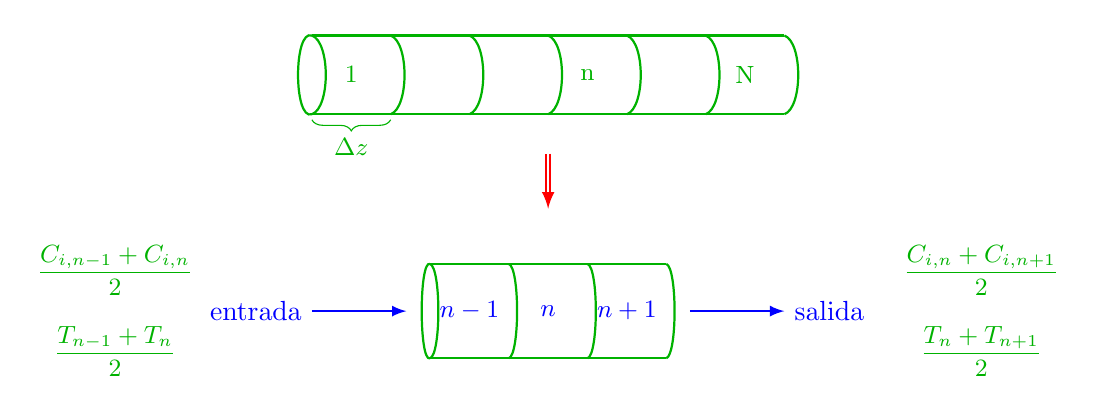
\begin{tikzpicture}[
            cylinder line/.style={draw=green!70!black, thick},
            label style/.style={green!70!black, font=\small},
            arrow style/.style={double, -latex, red, thick},
            eq style/.style={green!70!black, font=\small, align=center},
            blue label/.style={blue, font=\small}
        ]

        % --- CILINDRO SUPERIOR (VISIÓN GENERAL) ---
        \foreach \i/\txt in {0/1, 1/, 2/, 3/n, 4/, 5/N} {
                \coordinate (T\i) at (\i, 1);
                \coordinate (B\i) at (\i, 0);

                \ifnum\i<6
                    \draw[cylinder line] (T\i) -- ++(1,0);
                    \draw[cylinder line] (B\i) -- ++(1,0);
                \fi

                \draw[cylinder line] (T\i) to[out=-20, in=20, distance=0.25cm] (B\i);
                \node[label style] at (\i+0.5, 0.5) {\txt};
            }
        % Cierres elípticos
        \draw[cylinder line] (0,1) to[out=160, in=200, distance=0.25cm] (0,0);
        \draw[cylinder line] (6,1) to[out=-20, in=20, distance=0.25cm] (6,0);

        % Llave Delta z
        \draw [decorate, decoration={brace, amplitude=4pt, mirror, raise=2pt}, label style]
        (0,0) -- (1,0) node [midway, yshift=-12pt] {$\Delta z$};

        % --- FLECHA ROJA DE UNIÓN ---
        \draw[arrow style] (3,-0.5) -- (3,-1.2);

        % --- DETALLE DEL NODO (ZOOM ABAJO CON 3 SECCIONES) ---
        \begin{scope}[shift={(3, -2.5)}]
            % Definición de fronteras para 3 secciones
            % x=-1.5 (inicio), x=-0.5 (separación), x=0.5 (separación), x=1.5 (fin)

            % Líneas horizontales largas
            \draw[cylinder line] (-1.5, 0.6) -- (1.5, 0.6);
            \draw[cylinder line] (-1.5, -0.6) -- (1.5, -0.6);

            % Caras de las secciones
            \foreach \x/\labeltext in {-1.5/{n-1}, -0.5/{}, 0.5/{}, 1.5/{n+1}} {
            \draw[cylinder line] (\x, 0.6) to[out=-20, in=20, distance=0.15cm] (\x, -0.6);
            }

            % Cara inicial cerrada (izquierda)
            \draw[cylinder line] (-1.5, 0.6) to[out=160, in=200, distance=0.15cm] (-1.5, -0.6);

            % Etiquetas de las secciones centradas en cada tanque
            \node[blue label] at (-1, 0) {$n-1$};
            \node[blue label] at (0, 0) {$n$};
            \node[blue label] at (1, 0) {$n+1$};

            % Flechas de flujo centradas verticalmente
            \draw[blue, thick, -latex] (-3.0, 0) -- (-1.8, 0) node[pos=0, left] {entrada};
            \draw[blue, thick, -latex] (1.8, 0) -- (3.0, 0) node[pos=1, right] {salida};

            % --- ECUACIONES DESPLAZADAS ---
            % Izquierda (Entrada al nodo n)
            \node[eq style] at (-5.5, 0) {
                $\displaystyle \frac{C_{i,n-1} + C_{i,n}}{2}$ \\[10pt]
                $\displaystyle \frac{T_{n-1} + T_n}{2}$
            };

            % Derecha (Salida del nodo n)
            \node[eq style] at (5.5, 0) {
                $\displaystyle \frac{C_{i,n} + C_{i,n+1}}{2}$ \\[10pt]
                $\displaystyle \frac{T_n + T_{n+1}}{2}$
            };
        \end{scope}

    \end{tikzpicture}
    \caption{Esquematización en dinámico del reactor de flujo pistón.}
    \label{fig:rcfp-dinamico}
\end{figure}
\begin{flushleft}
    La forma de abordar su resolución consiste en aproximar el término diferencial axial como $\partial z\approx \Delta z$. De este modo, el reactor puede modelarse como una batería de tanques agitados ideales (RCMP) dispuestos en serie.\\

    Para ello, se divide el reactor en pequeños segmentos o “anillos” de longitud $\Delta z$. En cada uno de estos elementos diferenciales se aplican los balances de materia y energía como si se tratara de un reactor perfectamente agitado. Gracias a la capacidad de cálculo actual, es posible considerar valores de $\Delta z$ lo suficientemente pequeños como para obtener una aproximación muy precisa del comportamiento continuo del reactor.

    En consecuencia, los balances de componentes se formulan para cada uno de estos segmentos discretizados como:
\end{flushleft}
\begin{equation}
    \begin{alignedat}{2}
         & \underbrace{\Delta V \frac{d C_{i,n}}{d t}}_{\text{Acumulación}} &  & = \underbrace{F \cdot C_{i,n-1}}_{\text{Entrada}} - \underbrace{F \cdot C_{i,n}}_{\text{Salida}} + \underbrace{\Delta V \cdot r_{i,n}}_{\text{Generación}}
    \end{alignedat}
\end{equation}

\noindent Si a esta expresión la dividimos por $\Delta V$, obtendremos los balances de componentes genéricos, donde $i$ será el número de componentes y $n$ los segmentos en que hemos dividido el reactor.
\begin{equation}
    \frac{d C_{i,n}}{d t}=\frac{C_{i,n-1}-C_{i,n}}{\tau_n}+r_{i,n}
    \label{eq:rcfp-discreto}
\end{equation}

\noindent De forma análoga, para el balance de energía tenemos:
\begin{equation}
    \begin{alignedat}{2}
         & \text{1. Balance inicial:} \quad                                 &  & \Delta V \cdot \rho \cdot c_p \cdot \frac{dT_n}{dt} = F \cdot \rho \cdot c_p (T_{n-1} - T_n) + \Delta V \sum \Delta H_k \cdot r_k + Q(T)                                                                                                                                                                                                        \\[10pt]
         & \text{2. Dividir por } \textcolor{red}{\Delta V \rho c_p}: \quad &  & \frac{dT_n}{dt} = \frac{F \cdot \cancel{\rho \cdot c_p} (T_{n-1} - T_n)}{\textcolor{red}{\Delta V} \cdot \cancel{\textcolor{red}{\rho \cdot c_p}}} + \frac{\cancel{\Delta V} \sum \Delta H_k \cdot r_k}{\cancel{\textcolor{red}{\Delta V}} \cdot \textcolor{red}{\rho \cdot c_p}} + \frac{Q(T)}{\textcolor{red}{\Delta V \cdot \rho \cdot c_p}} \\[10pt]
         & \text{3. Simplificar términos:} \quad                            &  & \frac{dT_n}{dt} = \frac{F}{\Delta V} (T_{n-1} - T_n) + \frac{\sum \Delta H_k \cdot r_k}{\rho \cdot c_p} + \frac{Q(T)}{\Delta V \cdot \rho \cdot c_p}                                                                                                                                                                                            \\[10pt]
         & \text{4. Aplicar } \tau_n = \frac{\Delta V}{F}: \quad            &  & \frac{dT_n}{dt} = \frac{T_{n-1} - T_n}{\tau_n} + \frac{\sum \Delta H_k \cdot r_k}{\rho \cdot c_p} + \frac{Q(T)}{\Delta V \cdot \rho \cdot c_p}
    \end{alignedat}
\end{equation}

\nt{donde se tendria $P\cdot N$ balances de componente y $N$ balances de energia.}

\noindent Otros autores, como Fogler, proponen una formulación alternativa en la que el término convectivo no se evalúa únicamente en el nodo anterior \(n-1\), sino como un promedio entre nodos adyacentes, tal y como se muestra en la Figura \ref{fig:rcfp-dinamico}. De este modo, el balance de materia queda:
\vspace{1em}
\begin{equation}
    \Delta V \,\frac{d C_{i,n}}{d t}
    =
    \frac{F}{2}\left(C_{i,n-1}+C_{i,n}\right)
    -
    \frac{F}{2}\left(C_{i,n}+C_{i,n+1}\right)
    +
    \Delta V\, r_{i,n}
    \label{eq:rcfp-discreto2}
\end{equation}
\vspace{0.5em}
\noindent Expresándolo en términos del tiempo espacial \( \tau_n = \frac{\Delta V}{F} \), se obtiene la forma discreta:
\vspace{0.5em}

\begin{equation}
    \frac{d C_{i,n}}{d t}
    =
    \frac{C_{i,n-1}+C_{i,n}}{2\tau_n}
    -
    \frac{C_{i,n}+C_{i,n+1}}{2\tau_n}
    +
    r_{i,n}
    \label{eq:rcfp-discreto3}
\end{equation}

\vspace{0.5em}
\noindent De forma análoga, el balance de energía (entalpía) se escribe como:

\vspace{0.5em}

\begin{equation}
    \frac{dT_n}{dt}
    =
    \frac{T_{n-1}+T_n}{2\tau_n}
    -
    \frac{T_n+T_{n+1}}{2\tau_n}
    +
    \frac{\sum_k \Delta H_k \, r_{k,n}}{\rho \, c_p}
    +
    \frac{Q(T_n)}{\Delta V \, \rho \, c_p}
    \label{eq:rcfp-discreto4}
\end{equation}

\vspace{0.5em}

\noindent que, tras simplificación de los términos convectivos, puede expresarse como:

\vspace{0.5em}

\begin{equation}
    \frac{dT_n}{dt}
    =
    \frac{T_{n-1}-T_{n+1}}{2\tau_n}
    +
    \frac{\sum_k \Delta H_k \, r_{k,n}}{\rho \, c_p}
    +
    \frac{Q(T_n)}{\Delta V \, \rho \, c_p}
    \label{eq:rcfp-discreto5}
\end{equation}
\newpage
\section{Modelo de dispersión axial}
\begin{flushleft}
    El modelo de dispersión axial considera un reactor con mezcla radial perfecta pero axial parcial. Según la \textbf{Ley de Fick}, los gradientes de concentración activan un transporte difusivo que, al oponerse al flujo principal, genera una \textbf{retromezcla (backmixing)} de productos hacia la entrada, alejando al sistema del comportamiento ideal de flujo pistón.
\end{flushleft}
\begin{equation}
    \frac{c_n - c_{n-1}}{\Delta z}
    \;\xleftarrow{\text{Entrada}}\;
    \boxed{
        \frac{\partial C}{\partial t}
        =
        -\frac{\partial}{\partial z}
        \left( D \frac{\partial C}{\partial z} \right)
    }
    \;\xrightarrow{\text{Salida}}\;
    \frac{c_{n+1} - c_n}{\Delta z}
\end{equation}

\nt{Importante: Este fenómeno es significativo cuando la difusividad de los reactivos es pequeña. Si la difusividad fuera nula ($D=0$), el sistema trabajaría en condiciones ideales de Reactor de Flujo Pistón (RCFP).}

\subsubsection*{Parámetros Adimensionales}

\noindent el perfil de concentraciones se expresa en función de grupos adimensionales que cuantifican la desviación de la idealidad:

\begin{itemize}
    \item \textbf{Parámetros Adimensionales:}
\end{itemize}

\noindent
\begin{minipage}{0.5\textwidth}
    \centering
    \textbf{Módulo de dispersión ($N_D$)}
    \[ N_D = \frac{D}{v \cdot L} \]
\end{minipage}%
\begin{minipage}{0.5\textwidth}
    \centering
    \textbf{Número de Péclet ($Pe$)}
    \[ Pe = \frac{v \cdot L}{D} \]
\end{minipage}
\nt{siendo $D$ el coeficiente de difusión, $v$ la velocidad de paso (de la mezcla reaccionante) $L$ la longitud del reactor.}
\vspace{0.5cm}
\subsubsection*{Casos Límite}

\noindent El comportamiento del reactor depende del valor de $Pe$. En la figura \ref{fig:dispersion_mecanismo} se puede ver como funciona el mecanismo de dispersión axial y en la figura \ref{fig:dispersion_peclet} como varia en función del número de Péclet.

\begin{multicols}{2}
    \begin{enumerate}
        \item \textbf{Mezcla completa ($Pe=0$)}: $D \to \infty$. Perfil \textbf{aplanado} (comportamiento RTCA).
        \item \textbf{Flujo pistón ($Pe \to$ inf)}: $D=0$. Sin dispersión axial. Perfil \textbf{ideal} (RFP).
    \end{enumerate}
\end{multicols}

\begin{figure}[htbp]
    \centering
    % --- PRIMER SUBPLOT: Mecanismo de Dispersión ---
    \begin{subfigure}[b]{0.48\textwidth}
        \centering
        \begin{tikzpicture}[scale=0.9]
            % Ejes y etiquetas
            \draw[thick, green!70!black, ->] (0,0) -- (5.5,0) node[right, black] {$z$};
            \draw[thick, green!70!black, ->] (0,0) -- (0,3.5) node[above, black] {$C_i$};
            \node[below, green!70!black] at (0,0) {$0$};
            \node[below, green!70!black] at (5,0) {$L$};

            % --- PERFIL REACTIVO (R) ---
            \draw[ultra thick, blue] (0,3.2) .. controls (1,2) and (3,0.3) .. (5,0.25) node[right] {\textcolor{blue}{\textbf{R}}}
            node[pos=0.3, red, rotate=30] (puntoR1) {$+$}
            node[pos=0.45, red, rotate=30] (puntoR2) {$+$};

            % --- PERFIL PRODUCTO (P) ---
            \draw[ultra thick, black] (0,0.2) .. controls (1.5,0.5) and (3.5,2.2) .. (5,3.2) node[right] {\textbf{P}}
            node[pos=0.7, red, rotate=30] (puntoP1) {$+$}
            node[pos=0.85, red, rotate=30] (puntoP2) {$+$};

            % --- FLECHAS ---
            \draw[red, thick, -Stealth] (puntoR1.center) -- (puntoR2 |- puntoR1.center);
            \draw[red, thick, -Stealth] (puntoP2.center) -- (puntoP1 |- puntoP2.center);

            % Nota aclaratoria
            \node[anchor=north, font=\scriptsize, draw=gray!30, fill=gray!5, rounded corners, inner sep=4pt, text width=4.8cm, align=center] at (2.75, -0.6) {
                \textbf{Dispersión axial:} El aspa indica la posición local y la flecha el sentido del transporte difusivo neto.
            };
        \end{tikzpicture}
        \vspace{0.4cm}
        \caption{Mecanismo de dispersión y retromezcla local.}
        \label{fig:dispersion_mecanismo}
    \end{subfigure}%
    \hfill
    % --- SEGUNDO SUBPLOT: Perfiles según Pe ---
    \begin{subfigure}[b]{0.48\textwidth}
        \centering
        \begin{tikzpicture}
            \begin{axis}[
                    width=\textwidth,
                    height=5.8cm,
                    xlabel={Posición axial adim. ($z/L$)},
                    ylabel={Concentración adim. ($C/C_0$)},
                    xmin=0, xmax=1,
                    ymin=0, ymax=1.2,
                    % Leyenda dentro del gráfico (esquina superior derecha)
                    legend style={at={(0.97,0.97)}, anchor=north east, font=\tiny, row sep=-2pt},
                    grid=both,
                    grid style={line width=.1pt, draw=gray!10},
                    major grid style={line width=.2pt,draw=gray!50},
                ]

                % Caso Pe = 0 (RTCA -> perfil plano)
                \addplot[ultra thick, blue, dashed, domain=0:1, samples=2] {0.5};
                \addlegendentry{$Pe = 0$ (RTCA)}

                % Dispersión parcial: Pe bajo (más mezclado, caída suave)
                \addplot[ultra thick, orange, domain=0:1, samples=50] {0.7 * exp(-0.8*x)};
                \addlegendentry{$Pe$ bajo}

                % Dispersión parcial: Pe alto (menos mezclado, caída fuerte)
                \addplot[ultra thick, darkgreen, domain=0:1, samples=50] {0.9 * exp(-1.8*x)};
                \addlegendentry{$Pe$ alto}

                % Caso Pe -> infinito (RFP -> gradiente ideal)
                \addplot[ultra thick, red, domain=0:1, samples=100] {exp(-3.5*x)};
                \addlegendentry{\mbox{$Pe \to \infty$} (RFP)}


            \end{axis}
        \end{tikzpicture}
        \caption{Efecto del Número de Péclet ($Pe$) en el perfil de concentración.}
        \label{fig:dispersion_peclet}
    \end{subfigure}

    \caption{Análisis del modelo de dispersión axial.}
    \label{fig:dispersion_global}
\end{figure}

\begin{enumerate}
    \item \textbf{Balance de materia original (Discreto)}: Partimos del balance en un elemento de volumen $\Delta V$ para el nodo $n$, considerando transporte por flujo (convección), dispersión axial (difusión) y reacción química:
          \begin{equation}
              \Delta V \frac{dC_{i,n}}{dt} = F \cdot (C_{i,n-1} - C_{i,n}) + S \cdot D \cdot \left( \frac{C_{i,n-1} - C_{i,n}}{\Delta z} - \frac{C_{i,n} - C_{i,n+1}}{\Delta z} \right) + \Delta V r_{i,n}
          \end{equation}

    \item \textbf{Simplificación de la ecuación temporal}: Dividimos por $\Delta V$. Como $\Delta V = S \cdot \Delta z$, el coeficiente de dispersión se simplifica a $\frac{S \cdot D}{S \cdot \Delta z} = \frac{D}{\Delta z}$:
          \begin{equation}
              \frac{dC_{i,n}}{dt} = \frac{F}{\Delta V} (C_{i,n-1} - C_{i,n}) + \frac{D}{\Delta z} \left( \frac{C_{i,n-1} - 2C_{i,n} + C_{i,n+1}}{\Delta z} \right) + r_{i,n}
          \end{equation}

    \item \textbf{Definición de variables adimensionales}: Aplicamos las sustituciones para normalizar la expresión:
          \begin{multicols}{3}
              \begin{itemize}
                  \item $\bar{C}_i = \frac{C_i}{C_{i,0}}$
                  \item $\overline{\Delta z} = \frac{\Delta z}{L}$
                  \item $\theta = \frac{t}{\tau}$
              \end{itemize}
          \end{multicols}

    \item \textbf{Ecuación final adimensional}: Sustituyendo las variables y usando $\tau = \frac{L}{v}$, obtenemos la expresión final del modelo:
          \begin{equation}
              \frac{d\bar{C}_{i,n}}{d\theta} = \frac{\bar{C}_{i,n-1} - \bar{C}_{i,n}}{\overline{\Delta z}} + \frac{D}{v \cdot L} \left( \frac{\bar{C}_{i,n-1} - 2\bar{C}_{i,n} + \bar{C}_{i,n+1}}{\langle (\Delta z)^2 \rangle} \right) + \frac{L}{v \cdot C_{i,0}} \cdot r_{i,n}
          \end{equation}
\end{enumerate}

\vspace{0.3cm}
\nt{\textit{Nota: El término $\frac{D}{v \cdot L}$ corresponde al \textbf{Módulo de Dispersión axial ($N_D$)}, equivalente a $1/Pe$.}}
\section{Scilab}
\begin{table}[H]
    \centering
    \renewcommand{\arraystretch}{1.5}
    \begin{tabular}{|m{5cm}|m{3cm}|m{3cm}|m{4cm}|}
        \hline
        \rowcolor{teal!20}
        \textbf{Detalles Claves}                                                              & \textbf{Isotermo}               & \textbf{Adiabático}             & \textbf{No Adiabático / No Isotermo} \\
        \hline
        Obtener el estado estacionario                                                        & \hyperlink{qs:RCFP-1a}{RCFP-1a} & \hyperlink{qs:RCFP-1b}{RCFP-1b} & \hyperlink{qs:RCFP-1c}{RCFP-1c}      \\
        \hline
        Reactores adiabáticos en serie con enfriamiento intermedio (Optimización de longitud) &                                 & \hyperlink{qs:RCFP-1d}{RCFP-1d} &                                      \\
        \hline
        Proceso con recirculación (Optimizar fracción de recirculación)                       & \hyperlink{qs:RCFP-2}{RCFP-2}   &                                 &                                      \\
        \hline
    \end{tabular}
    \caption{Clasificación de los ejercicios resueltos del RCFP}
    \label{tab:clasificacion_rcfp}
\end{table}

\hypertarget{qs:RCFP-1a}{}\qs{RCFP-1a}{El equilibrio químico:
    $$ A + B \rightleftharpoons C $$
    Factor preexponencial de Arrhenius = $1.75 \times 10^8$ L/(mol$\cdot$h)\\
    Factor preexponencial de Van't Hoff = $8.25 \times 10^{-22}$ L/mol\\
    Energía de activación = $62350$ J/mol\\
    Entalpía de reacción = $-136400$ J/mol

    Se lleva a cabo en condiciones isotermas a 310 K en un reactor tubular de 800 dm de longitud y 3 dm de diámetro alimentado por 50 L/h de los compuestos A, B y C a concentración 1.5, 2.0 y 0.1 mol/L, respectivamente. La mezcla reaccionante presenta una densidad de 1150 g/L y una capacidad calorífica de 3.8 J/(g$\cdot$K).

    \begin{enumerate}[label={\alph*)}]
        \item Obtener el estado estacionario del proceso.
    \end{enumerate}}
\begin{minted}[fontsize=\small, linenos]{scilab}
clear; clc;
// RCFP-1a.sce
// A + B <=> C
// Isotermo
// Estado estacionario

// EQUIVALENCIA
// RCFP                         RDMP             
// Estado estacionario          Dinámica         
// Tiempo de residencia         Tiempo           
// Entrada                      Valores iniciales        
// Salida                       Valores finales                   

// SISTEMA DE ECUACIONES DIFERENCIALES
function dxdtau = f(tau,x)
    // Variables diferenciales
    CA = x(1)
    CB = x(2)
    CC = x(3)
    // Ecuación de Arrhenius
    kd = kd0*exp(-E/(R*T))
    // Ecuación de Van't Hoff
    Keq = Keq0*exp(-H/(R*T))
    // Velocidad de reacción
    // r = rd - ri = kd*CA*CB - ki*CC = kd*CA*CB - kd*CC/Keq
    r = kd*(CA*CB - CC/Keq)
    // Balance de materia para A
    // RDMP: d(V*CA)dt = -r*V 
    dCAdtau = -r
    // Balance de materia para B
    // RDMP: d(V*Cb)dt = -r*V 
    dCBdtau = -r
    // Balance de materia para C
    // RDMP: d(V*Cc)dt = r*V 
    dCCdtau =  r
    // Derivadas
    dxdtau(1) = dCAdtau
    dxdtau(2) = dCBdtau
    dxdtau(3) = dCCdtau
endfunction

// CONSTANTES
kd0 = 1.75E8; // L/(mol*h)
E = 62350; // J/mol
Keq0 = 8.25E-22; // L/mol
H = -136400; // J/mol
R = 8.314; // J/(mol*K)
RHO = 1150; // g/L
CP = 3.8; // J/(g*K)
F = 50; // L/h 
D = 3; // dm
L = 800; // dm
V = %pi/4*D^2*L // L
TAU = V/F // h

T = 310; // K

// ENTRADA
CA0 = 1.5; CB0 = 2; CC0 = 0.1; // mol/L
x0 = [CA0;CB0;CC0];

// TIEMPO DE RESIDENCIA
N = 800 ; tau = 0:TAU/N:TAU; // h
l = 0:L/N:L; // dm

// RESOLVER
x = ode(x0,0,tau,f);
CA = x(1,:); CAs = CA($)
CB = x(2,:); CBs = CB($) 
CC = x(3,:); CCs = CC($)
XA = 1 - CA/CA0; XAs = XA($)
//Det la conversion a mitad del reactor
Xam = XA(L/2) // o $/2
disp('la conversion en mitad del reactor es' ,Xam);

// GRÁFICAS
scf(1); clf(1); 
plot(l,CA,l,CB,l,CC);
xgrid; xlabel('l'); legend('CA','CB','CC',-2,%f);

scf(2); clf(2); 
plot(l,XA,'m');
plot(L/2,Xam,'mo','markersize',6);
xgrid; xlabel('l'); legend('XA',-2,%f);
disp('V' ,V);
disp('TAU' ,TAU);
disp('CA' ,CAs);
disp('CB' ,CBs);
disp('CC' ,CCs);
disp('XA' ,XAs);

//TODO Determinar la conversion a mitad del reactor 
\end{minted}

\hypertarget{qs:RCFP-1b}{}\qs{RCFP-1b}{El equilibrio químico:
    $$ A + B \rightleftharpoons C $$
    Factor preexponencial de Arrhenius = $1.75 \times 10^8$ L/(mol$\cdot$h)\\
    Factor preexponencial de Van't Hoff = $8.25 \times 10^{-22}$ L/mol\\
    Energía de activación = $62350$ J/mol\\
    Entalpía de reacción = $-136400$ J/mol

    Se lleva a cabo en condiciones adiabáticas en un reactor tubular de 800 dm de longitud y 3 dm de diámetro alimentado por 50 L/h a 310 K de los compuestos A, B y C a concentración 1.5, 2.0 y 0.1 mol/L, respectivamente. La mezcla reaccionante presenta una densidad de 1150 g/L y una capacidad calorífica de 3.8 J/(g$\cdot$K).

    \begin{enumerate}[label={\alph*)}]
        \item Obtener el estado estacionario del proceso.
    \end{enumerate}}
\begin{minted}[fontsize=\small, linenos]{scilab}
clear; clc;
// RCFP-1b.sce
// A + B <=> C
// Adiabático
// Estado estacionario

// SISTEMA DE ECUACIONES DIFERENCIALES
function dxdtau = f(tau,x)
    // Variables diferenciales
    CA = x(1)
    CB = x(2)
    CC = x(3)
    T  = x(4)
    // Ecuación de Arrhenius
    kd = kd0*exp(-E/(R*T))
    // Ecuación de Van't Hoff
    Keq = Keq0*exp(-H/(R*T))
    // Velocidad de reacción
    // r = rd - ri = kd*CA*CB - ki*CC = kd*CA*CB - kd*CC/Keq
    r = kd*(CA*CB - CC/Keq)
    // Balance de materia para A
    // RDMP: d(V*CA)dt = -r*V 
    dCAdtau = -r
    // Balance de materia para B
    // RDMP: d(V*Cb)dt = -r*V 
    dCBdtau = -r
    // Balance de materia para C
    // RDMP: d(V*Cc)dt = r*V 
    dCCdtau =  r
    // Balance de energía
    // RDMP: d(V*RHO*CP*T)dt = -H*r*V
    dTdtau = -H*r/(RHO*CP) 
    // Derivadas
    dxdtau(1) = dCAdtau
    dxdtau(2) = dCBdtau
    dxdtau(3) = dCCdtau
    dxdtau(4) = dTdtau
endfunction

// CONSTANTES
kd0 = 1.75E8; // L/(mol*h)
E = 62350; // J/mol
Keq0 = 8.25E-22; // L/mol
H = -136400; // J/mol
R = 8.314; // J/(mol*K)
RHO = 1150; // g/L
CP = 3.8; // J/(g*K)
F = 50; // L/h 
D = 3; // dm
L = 800; // dm
V = %pi/4*D^2*L // L
TAU = V/F // h

// ENTRADA
CA0 = 1.5; CB0 = 2; CC0 = 0.1; // mol/L
T0 = 310; // K
x0 = [CA0;CB0;CC0;T0];

// TIEMPO DE RESIDENCIA
N = 800; tau = 0:TAU/N:TAU; // h
l = 0:L/N:L; // dm

// RESOLVER
x = ode(x0,0,tau,f);
CA = x(1,:); CAs = CA($);
CB = x(2,:); CBs = CB($);
CC = x(3,:); CCs = CC($);
T  = x(4,:); Ts  = T($);
XA = 1 - CA/CA0; XAs = XA($);
s = 8; // número de segmentos
s2ini = T(l=1*L/8);
s2fin = T(l=2*L/8);
if s2ini == s2fin then
    disp('El reactor no esta progresando y su diferencia de temperatura es cero')
else
    disp('El reactor esta progresando',(s2fin-s2ini), 'K')
end
// GRÁFICAS
scf(1); clf(1); 
plot(l,XA,'m');
xgrid; xlabel('l'); legend('XA',-2,%f);

scf(2); clf(2); 
plot(l,T,'r');
xgrid; xlabel('l'); legend('T',-2,%f);

scf(3); clf(3); 
plot(T,XA,'mo-');
xgrid; xlabel('T'); legend('XA',-2,%f);

//TODO si dividimos el reactor en 8 segmentos, aumenta la temperatura en el segundo segmento?
\end{minted}

\hypertarget{qs:RCFP-1c}{}\qs{RCFP-1c}{El equilibrio químico:
    $$ A + B \rightleftharpoons C $$
    Factor preexponencial de Arrhenius = $1.75 \times 10^8$ L/(mol$\cdot$h)\\
    Factor preexponencial de Van't Hoff = $8.25 \times 10^{-22}$ L/mol\\
    Energía de activación = $62350$ J/mol\\
    Entalpía de reacción = $-136400$ J/mol

    Se lleva a cabo en condiciones no adiabáticas en un reactor tubular de 800 dm de longitud y 3 dm de diámetro alimentado por 50 L/h a 310 K de los compuestos A, B y C a concentración 1.5, 2.0 y 0.1 mol/L, respectivamente. El reactor está refrigerado por una camisa por la que circula un fluido a 310 K, con un coeficiente global de transmisión de calor de 900 J/(dm$^2\cdot$h$\cdot$K). La mezcla reaccionante presenta una densidad de 1150 g/L y una capacidad calorífica de 3.8 J/(g$\cdot$K).

    \begin{enumerate}[label={\alph*)}]
        \item Obtener el estado estacionario del proceso.
    \end{enumerate}}
\begin{minted}[fontsize=\small, linenos]{scilab}
clear; clc;
// RCFP-1c.sce
// A + B <=> C
// No adiabático
// Estado estacionario

// SISTEMA DE ECUACIONES DIFERENCIALES
function dxdtau = f(tau,x)
    // Variables diferenciales
    CA = x(1)
    CB = x(2)
    CC = x(3)
    T  = x(4)
    // Ecuación de Arrhenius
    kd = kd0*exp(-E/(R*T))
    // Ecuación de Van't Hoff
    Keq = Keq0*exp(-H/(R*T))
    // Velocidad de reacción
    // r = rd - ri = kd*CA*CB - ki*CC = kd*CA*CB - kd*CC/Keq
    r = kd*(CA*CB - CC/Keq)
    // Balance de materia para A
    // RDMP: d(V*CA)dt = -r*V 
    dCAdtau = -r
    // Balance de materia para B
    // RDMP: d(V*Cb)dt = -r*V 
    dCBdtau = -r
    // Balance de materia para C
    // RDMP: d(V*Cc)dt = r*V 
    dCCdtau =  r
    // Balance de energía
    // RDMP: d(V*RHO*CP*T)dt = -H*r*V - Q = -H*r*V - U*A*(T-TJ)
    // RDMP: dTdt = -H*r/(RHO*CP) - U*A*(T-TJ)/(V*RHO*CP)
    // A/V = %pi*D*L / (%pi/4*D^2*L) = 4/D 
    dTdtau = -H*r/(RHO*CP) - 4*U*(T-TJ)/(D*RHO*CP)
    // Derivadas
    dxdtau(1) = dCAdtau
    dxdtau(2) = dCBdtau
    dxdtau(3) = dCCdtau
    dxdtau(4) = dTdtau
endfunction

// CONSTANTES
kd0 = 1.75E8; // L/(mol*h)
E = 62350; // J/mol
Keq0 = 8.25E-22; // L/mol
H = -136400; // J/mol
R = 8.314; // J/(mol*K) 
RHO = 1150; // g/L
CP = 3.8; // J/(g*K)
F = 50; // L/h 
D = 3; // dm
L = 800; // dm
V = %pi/4*D^2*L // L
TAU = V/F // h

U = 900; // J/(dm2*h*K)
TJ = 310; // K
//! hacer un bucle para ver como varia la conversion con la temperatura de refrigeracion para buscar optimo
//! de forma que aumente el rango si aumenta la temperatura o disminuye la t si aumenta la conversion con el signo de derivda
//! para calcular el optimo tal que sea < tol 
// ENTRADA
CA0 = 1.5; CB0 = 2; CC0 = 0.1; // mol/L
T0 = 310; // K
x0 = [CA0;CB0;CC0;T0];

// TIEMPO DE RESIDENCIA
tau = 0:TAU/100:TAU; // h
l = 0:L/100:L; // dm

// RESOLVER
x = ode(x0,0,tau,f);
CA = x(1,:); CAs = CA($) 
CB = x(2,:); CBs = CB($) 
CC = x(3,:); CCs = CC($)
T  = x(4,:); Ts  = T($)
XA = 1 - CA/CA0; XAs = XA($)

// GRÁFICAS
scf(1); clf(1); 
plot(l,XA,'m');
xgrid; xlabel('l'); legend('XA',-2,%f);

scf(2); clf(2); 
plot(l,T,'r');
xgrid; xlabel('l'); legend('T',-2,%f);

scf(3); clf(3); 
plot(T,XA,'mo-');
xgrid; xlabel('T'); legend('XA',-2,%f);

scf(4);
plot(TJ, XAs,'mo');
xgrid; xlabel('TJ'); ylabel('XAs');
\end{minted}

\hypertarget{qs:RCFP-1d}{}\qs{RCFP-1d}{El equilibrio químico:
    $$ A + B \rightleftharpoons C $$
    Factor preexponencial de Arrhenius = $1.75 \times 10^8$ L/(mol$\cdot$h)\\
    Factor preexponencial de Van't Hoff = $8.25 \times 10^{-22}$ L/mol\\
    Energía de activación = $62350$ J/mol\\
    Entalpía de reacción = $-136400$ J/mol

    Se lleva a cabo en un sistema de dos reactores tubulares adiabáticos en serie con un enfriamiento intermedio. El sistema completo tiene una longitud equivalente de 800 dm y 3 dm de diámetro, y es alimentado por 50 L/h a 310 K de los compuestos A, B y C a concentración 1.5, 2.0 y 0.1 mol/L, respectivamente. Entre ambos reactores se enfría la mezcla hasta la temperatura inicial de 310 K. La mezcla reaccionante presenta una densidad de 1150 g/L y una capacidad calorífica de 3.8 J/(g$\cdot$K).

    \begin{enumerate}[label={\alph*)}]
        \item Obtener el estado estacionario del proceso y optimizar la longitud del primer reactor.
    \end{enumerate}}
\begin{minted}[fontsize=\small, linenos]{scilab}
clear; clc;
// RCFP-1d.sce
// A + B <=> C
// Adiabático
// Estado estacionario
// 2 reactores con enfriamiento intermedio

// SISTEMA DE ECUACIONES DIFERENCIALES
function dxdtau = f(tau,x)
    // Variables diferenciales
    CA = x(1)
    CB = x(2)
    CC = x(3)
    T  = x(4)
    // Ecuación de Arrhenius
    kd = kd0*exp(-E/(R*T))
    // Ecuación de Van't Hoff
    Keq = Keq0*exp(-H/(R*T))
    // Velocidad de reacción
    // r = rd - ri = kd*CA*CB - ki*CC = kd*CA*CB - kd*CC/Keq
    r = kd*(CA*CB - CC/Keq)
    // Balance de materia para A
    // RDMP: d(V*CA)dt = -r*V 
    dCAdtau = -r
    // Balance de materia para B
    // RDMP: d(V*Cb)dt = -r*V 
    dCBdtau = -r
    // Balance de materia para C
    // RDMP: d(V*Cc)dt = r*V 
    dCCdtau =  r
    // Balance de energía
    // RDMP: d(V*RHO*CP*T)dt = -H*r*V
    dTdtau = -H*r/(RHO*CP) 
    // Derivadas
    dxdtau(1) = dCAdtau
    dxdtau(2) = dCBdtau
    dxdtau(3) = dCCdtau
    dxdtau(4) = dTdtau
endfunction

// CONSTANTES
kd0 = 1.75E8; // L/(mol*h)
E = 62350; // J/mol
Keq0 = 8.25E-22; // L/mol
H = -136400; // J/mol
R = 8.314; // J/(mol*K)
RHO = 1150; // g/L
CP = 3.8; // J/(g*K)
F = 50; // L/h 
D = 3; // dm
L = 800; // dm

// *********
// REACTOR 1
// *********

// CONSTANTES
L1 = 400; // dm
V1 = %pi/4*D^2*L1 // L
TAU1 = V1/F // h

// ENTRADA
CA0 = 1.5; CB0 = 2; CC0 = 0.1; // mol/L
T0 = 310; // K
x01 = [CA0;CB0;CC0;T0];

// TIEMPO DE RESIDENCIA
N =400; tau1 = 0:TAU1/N:TAU1; // h
l1 = 0:L1/N:L1; // dm

// RESOLVER
x1 = ode(x01,0,tau1,f);
CA1 = x1(1,:); CA1s = CA1($) 
CB1 = x1(2,:); CB1s = CB1($) 
CC1 = x1(3,:); CC1s = CC1($)
T1  = x1(4,:); T1s  = T1($)
XA1 = 1 - CA1/CA0; XA1s = XA1($)


d2XA1 = diff(XA1,2); // segunda derivada de XA1
indexXA1 = find(d2XA1(1:$-1).*d2XA1(2:$) < 0) + 1; // índice de los puntos de inflexión
lli = l1(indexXA1);
XA1i = XA1(indexXA1);
disp('el cambio de reactor optimo es a la longitud = ', lli, 'dm' , ' y la conversion = ', XA1i, 'mol/L')
L3 = lli; // dm
V3 = %pi/4*D^2*L3 // L
TAU3 = V3/F // h
tau3 = 0:TAU3/N:TAU3
l3 = 0:L3/N:L3; // dm
// RESOLVER
x3 = ode(x01,0,tau3,f);
CA3 = x3(1,:); CA3s = CA3($);
CB3 = x3(2,:); CB3s = CB3($);
CC3 = x3(3,:); CC3s = CC3($);
T3  = x3(4,:); T3s  = T3($);
XA3 = 1 - CA3/CA0; XA3s = XA3($);


// *********
// REACTOR 2
// *********

// CONSTANTES
L2 = L - lli; // dm
V2 = %pi/4*D^2*L2 // L
TAU2 = V2/F // h

// ENTRADA
// x02 = [CA1s;CB1s;CC1s;T0];  // Enfriamiento: T1s => T0 si fuera otra cosa en vez de T0 se pondria su valor
x02 = [CA3s;CB3s;CC3s;T0];  //*optimizado el otro era a mitad del reactor 
// TIEMPO DE RESIDENCIA
N =400; tau2 = 0:TAU2/N:TAU2; // h
l2 = 0:L2/N:L2; // dm
l2s = l2 + lli; // dm, para que la grafica de l2 empiece desde el final de l1

// RESOLVER
x2 = ode(x02,0,tau2,f);
CA2 = x2(1,:); CA2s = CA2($) 
CB2 = x2(2,:); CB2s = CB2($) 
CC2 = x2(3,:); CC2s = CC2($)
T2  = x2(4,:); T2s  = T2($)
XA2 = 1 - CA2/CA0; XA2s = XA2($) //! se pone CA2/Ca0 por que es la conversion respecto a la entrada inicial para ver la conversion total del reactor y no de forma individual   

disp('la conversion final del reactor 2 es = ', XA2s, 'mol/L')
// GRÁFICAS
scf(1); clf(1); 
plot(l3,XA3,'m',l2s,XA2,'m--');
xgrid; xlabel('l'); legend('XA1','XA2',-2,%f); 

scf(2); clf(2); 
plot(l3,T3,'r',l2s,T2,'r--');
xgrid; xlabel('l'); legend('T1','T2',-2,%f); 

scf(3); clf(3); 
plot(T3,XA3,'mo-',T2,XA2,'m.-');
xgrid; xlabel('T'); legend('XA1','XA2',-2,%f); 

scf(4);
plot(L1, XA2s,'mo');
xgrid; xlabel('L1'); ylabel('XA2s'); 
m=-RHO*CP/H*CA0; // pendiente teorica de la recta de enfriamiento
m2= (XA1s-0)/(T1s-T0); // pendiente de la recta de enfriamiento
m3 = (XA2s-XA1s)/(T2s-T0); // pendiente de la recta de enfriamiento
if m2 == m3 & m2 == m then //! cambiar el disp
    disp('El reactor esta progresando',(s2fin-s2ini), 'K')
else
    disp('El reactor no esta progresando y su diferencia de temperatura es cero')
end
//dxa/dtau = r/cao
//dxa/dtau = (1/cao)/(-H*r/(RHO*CP)) =-rho*CP/H*CA0* por eso ambas rectas son cortantes 
//buscar punto de inflexion 


scf(1); plot(lli,XA1i,'ro-');
//despues usar ese punto para calcular la conversiona al cambiar la L 
\end{minted}

\hypertarget{qs:RCFP-2}{}\qs{RCFP-2}{La reacción elemental e isoterma:
    $$ A + B \rightarrow 2B $$
    Con constante cinética $k = 1$ L/(mol$\cdot$h), se lleva a cabo en un proceso con recirculación. El sistema consta de un reactor tubular de 12 dm de longitud y 1 dm de diámetro. La alimentación fresca es de 5 L/h con una concentración de 2 mol/L de A y 0.01 mol/L de B. Parte de la corriente de salida se recircula a la entrada del reactor, con una relación de recirculación de $R = 0.1$.

    \begin{enumerate}[label={\alph*)}]
        \item Obtener el estado estacionario del proceso con el método del punto fijo.
        \item Optimizar la fracción de recirculación.
    \end{enumerate}}
\begin{minted}[fontsize=\small, linenos]{scilab}
clear; clc;
// RCFP-2.sce
// A + B => 2 B
// Isotermo
// Estado estacionario
// Recirculación 


// SISTEMA DE ECUACIONES DIFERENCIALES
function dxdtau = f(tau,x)
    // Variables diferenciales
    CA = x(1)
    CB = x(2)
    // Velocidad de reacción
    r = k*CA*CB
    // Balance de materia para A
    // RDMP: d(V*CA)dt = -r*V
    dCAdtau = -r
    // Balance de materia para B
    // RDMP: d(V*CB)dt = (-r + 2*r)*V
    dCBdtau = r   
    dxdtau(1) = dCAdtau
    dxdtau(2) = dCBdtau 
endfunction

// CONSTANTES
F =  5; // L/h
L =  12; // dm
D = 1; // dm
V = %pi/4*D^2*L // L
R = 0.1 ;
TAU = V/(F*(1+R))  // h
k = 1; // L/(mol·h)
CA0 = 2; // mol/L
CB0 = 0.01; // mol/L
x0 = [CA0;CB0];

// TIEMPO DE RESIDENCIA
N = 1000 ; tau = 0:TAU/N:TAU; // h
l = 0:L/N:L; // dm

// SOLUCIÓN SUPUESTA
CAsguess = 2; CBsguess = 0.01; // mol/L
xsguess = [CAsguess;CBsguess];

imax = 20;
tol = 1E-5;

for i = 1:imax
    
    i
    
    // Balance al mezclador
    // F*CA0 + F*R*CAsguess = F*(1+R)*CAe
    // F*CB0 + F*R*CBsguess = F*(1+R)*CBe
    // CAe = (CA0 + R*CAsguess)/(1+R)
    // CBe = (CB0 + R*CBsguess)/(1+R)
    xe = (x0 + R*xsguess)/(1+R);

    // RESOLVER
    x = ode(xe,0,tau,f);
    xs = x(:,$)
    
    err = abs(xs-xsguess);
    
    if err < tol then
        break
    else
        xsguess = xs;
    end

end

i;
CA = x(1,:); CAs = xs(1);
CB = x(2,:); CBs = xs(2);
disp('la concentracion final de A es:' +string(CAs)), disp('la concentracion final de B es:' +string(CBs));
scf(1); clf(1);
plot(l,CA,l,CB);
xgrid; xlabel('l'); legend('CA','CB',-2,%f);

scf(2);
plot(R,CAs,'o');
xgrid; xlabel('R'); ylabel('CAs');


//! hacer una segunda parte donde busque el optimo con R aumentandola 
\end{minted}

\qs{RCFP-2022-O}{El equilibrio químico

	A + B  $\rightleftarrows$  C
	
	Factor preexponencial de Arrhenius = 1.8E8 m$^3$/(kmol$\cdot$h)\\
	Factor preexponencial de Van't Hoff = 8.2E-22 m$^3$/kmol\\
	Energía de activación = 6.2E4 kJ/kmol\\
	Entalpía de reacción = -1.4E5 kJ/kmol

	se lleva a cabo en disolución acuosa y régimen adiabático en 3 reactores tubulares en serie de 20 m de longitud y 0.25 m de diámetro entre los que se sitúan 2 enfriadores con una potencia de 1000 kJ/h.

	\begin{enumerate}[label=\bfseries\scriptsize\protect\circled{\footnotesize\Alph*}]
		\item Obtener el estado estacionario del proceso considerando que el primer reactor es alimentado por 0.05 m$^3$/h a 310 K de los compuestos A y B a concentración 2 kmol/m$^3$
		\item Optimizar la potencia de enfriamiento
	\end{enumerate}
}

\qs{RCFP-2024-O}{En un reactor continuo tubular 30 m de largo y 0.25 m de diámetro, alimentado por una corriente de 0.5 m$^3$/min con 1500 mol/m$^3$ del compuesto A a 310 K, se lleva a cabo una reacción química exotérmica con entalpía de reacción = -4.1E5 J/mol

	A $\Rightarrow$ B\\
	k = 1.2E6$\cdot$exp(-5000/T) min$^{-1}$

	Considerando una densidad = 950 kg/m$^3$, una capacidad calorífica = 3.5E3 J/(kg$\cdot$K) y que el reactor dispone de una camisa a 280 K con un coeficiente global de transmisión de calor de 6.5E4 J/(min$\cdot$m$^2\cdot$K):

	\begin{enumerate}[label={\alph*)}]
		\item Obtener la conversión y la temperatura a lo largo del reactor en estado estacionario
		\item Localizar el punto de inflexión de la curva de conversión
		\item Determinar durante cuánta longitud la temperatura es superior a 420 K
	\end{enumerate}
}

\qs{RCFP-UNK}{La siguiente reacción química se lleva a cabo en fase líquida acuosa en una batería de 2 reactores continuos flujo pistón en serie de 2500 L cada uno:

	$A + B \rightleftarrows P$

	$k_d = 2\text{E}8 \cdot \exp(-7500/T) \text{ L/(mol}\cdot\text{h)}$\\
	$K_{eq} = 8\text{E-}22 \cdot \exp(16400/T) \text{ L/mol}$\\
	$\Delta H = -150000 \text{ J/mol}$

	Al primer reactor se alimentan 50 L/h a 300 K con 2 mol/L del compuesto A y 2 mol/L del compuesto B. Al segundo reactor se alimenta la salida del primero tras ser enfriada 25 K.

	Empleando Scilab, estudiar el estado estacionario del proceso aportando script, salida en consola, gráficas y comentarios.
}

\qs{RCFP-UNK-2}{En un reactor tubular continuo de 2 dm de diámetro tiene lugar la reacción de equilibrio en fase líquida

	A + B $\rightleftarrows$ C
	
	Factor preexponencial (Arrhenius) = 1.8E8 L/(mol$\cdot$h)\\
	Factor preexponencial (van't Hoff) = 8E-22 L/mol\\
	Energía de activación = 6.25E4 J/mol\\
	Entalpía de reacción = -1.5E5 J/mol

	El reactor es alimentado por 0.1 L/h de 1 mol A/h y 1 mol B/h a 310 K. Dispone de una camisa a 300 K que refrigera el reactor con un coeficiente de 10 J/(dm$^2\cdot$h$\cdot$K).

	\begin{enumerate}[label={\alph*)}]
		\item Considerando un tiempo de residencia de 1000 h, calcular el estado estacionario del reactor.
		\item Localizar el 50\% de conversión.
		\item Localizar la temperatura máxima.
	\end{enumerate}

	Asumir, cuando sea necesario, las propiedades físicas del agua.
}
